\section{Experiments with Synthetic Data}

%
%\subsection{Synthetic Data}
%
%We use synthetic data to illustrate the strengths and weaknesses of different methods by varying one independent
%dataset and tracking the performance metrics of each method:
%\begin{enumerate}
%  \item When do other methods outperform simple majority voting? Show performance against worker accuracy.
%  Similar experiments were carried out with a different set of baselines in \cite{Simpson2014Thesis}, Section 2.5.2, with all workers having similar accuracies, and Section 2.5.4, where some workers are noisy and others are highly accurate. Here, we vary the average accuracy of workers, with lower average accuracy leading to more diversity between workers. Analyse whether the full IBCC confusion matrix offers benefits over MACE due to worker accuracy varying between classes when accuracy is lower. 
%  \item How well do MACE, IBCC, and seq-BCC handle worker bias? Show performance against worker bias toward one class. This is a comparable experiment to \cite{Simpson2014Thesis}, Section 2.5.3, which notably does not include MACE.
%  \item How well does each method handle data sparsity? (a) Vary the amount of observations per worker. Expect MACE to perform well, seq-BCC may suffer from the larger confusion matrix. (b) Vary the number of observations per data point. 
%  \item Do MACE and IBCC still work with unbalanced datasets? Test with unbalanced class distributions, i.e. starting from $p(B) = p(I) = p(O) = .3$, decrease
%  $p(B)$ and $p(I)$ until $p(O) = .99$.
%\end{enumerate}
%In each case, we use a set of default values for the variables that are not currently being tested. These are
% chosen so that all methods perform well (e.g. 90\% accuracy) under the best conditions of the test. E.g. for the test where we vary worker accuracy, we set bias and sparsity to be low so that the performance of all methods is good when workers are 80\% accurate.
%
%For all methods except seq-BCC, we compute performance metrics both before and after the valid annotation post-processing step, which is required to ensure that I tokens do not follow O tokens.
%
%Performance metrics:
%\begin{enumerate}
%  \item Metrics that evaluate the quality of the most probable class labels: recall, precision and F1-score (of B class and I class separately), accuracy (mean over classes)
%  \item Metrics that evaluate the confidence values output by the models: area under ROC curve or AUC (separate for B and I classes), and cross entropy error %or brier score (mean over classes)
%  \item Annotation count error: the mean difference between the number of annotations produced by the model and the true number.
%  \item Number of invalid labels that must be corrected by post-processing.
%  \item Mean length of annotations compared to the ground truth: show whether some methods find annotation fragments.
%\end{enumerate}
%
%We also evaluate the competence scores estimated by each method. First, we compute the ground truth from the 
%synthetic confusion matrices. We use a weighted average over classes (weighted by class frequency) to produce the 
%overall worker accuracy. Then, we compute accuracy from seq-BCC, MACE and IBCC using similar methods. 
%For each method, we can compute the mean and STD of cross entropy error between the estimated and the ground truth
% confusion matrices. We then reproduce the plots described above, but showing the cross entropy error for the 
% competence estimates. 

%\subsection{Real-world Data}
%
%We investigate the performance on some real datasets to show how well the methods work when combining real workers. Besides the performance metrics mentioned above, we also quantitatively analyse examples of where seq-BCC outperforms other methods to show where they may have trouble forming valid or grammatically correct annotations, e.g. where the starting token is incorrect. 
%Ideally, we would also analyse whether the annotations produced are grammatically sensible, e.g. if there is conflict between workers about where an annotation should start, the method should choose one valid start point, not an invalid start point that lies in between. These points can be evaluated by computing:
%\begin{enumerate}
%\item The percentage of "sensible" annotations, as judged by an expert for the task. For tasks where this data is not available, we can use the following metrics to gauge annotation quality.
%\item The percentage of each method's annotations that have an exact match in the gold standard (exact annotation precision)
%\item The percentage of gold standard annotations that have an exact match in the method's output (exact annotation recall)
%\item Mean and variance of no. tokens difference to nearest annotation; this is averaged over the annotations, rather than the number of tokens, so gives a greater indication of how well they matched the gold standard.
%\end{enumerate}

We run several method comparisons using two NLP datasets to test whether the quality of aggregated labels is 
improved by (a) the more sophisticated worker models described in Section \ref{sec:model},
(b) the inclusion of text features into the graphical model or (c) a Bayesian approach. 
We further test whether Bayesian approach facilitates more efficient active learning of sequential annotations from crowds and whether integrating the LSTM into the ensemble of annotators improves performance further.
Our experiments consist of three tasks: (1) aggregating crowdsourced labels, (2) training the LSTM sequence tagger of Lample et al. ~\shortcite{lample2016} using aggregated labels, and (3) actively selecting batches of documents for crowdsourced annotation.
 
\section{Experiments with Real Data}
 
\section{Datasets}

We use two datasets containing both crowdsourced sequential annotations and gold annotations. 
The \emph{NER} dataset contains $1,393$ English documents from the CoNLL 2003 named-entity recognition dataset
~\cite{conll_ner_2003}, all of which contain gold labels for four named entity categories (PER, LOC, ORG, MISC). Of these, we use crowdsourced labels provided by \cite{rodrigues2014} for $415$ documents.
We also test on the \emph{PICO} dataset, introduced by Nguyen et al. ~\cite{nguyen2017aggregating},
containing $4,740$ medical paper abstracts, all of which have been 
annotated by a crowd to indicate text spans that identify the population enrolled in a clinical trial. There are gold labels for $191$ documents.

\section{Evaluation metrics}

For NER we use the established CoNLL 2003 F1-score, which is computed at the level of annotated spans that must match exactly to be considered correct. This measure is intuitive because complete named entities must be marked to be of value. For PICO, we use the relaxed F1-measure defined in ~\cite{nguyen2017aggregating}, which counts the matching fractions of spans when computing precision and recall. 
%We additionally compute the root mean squared error in the span lengths, i.e. the difference between the  % actually it's not quite that. We computed the difference in mean span lengths. This is already captured by F1 score for pico and better described by the span-level-precision and recall. Our metric might be more if we didn't take the absolute so we could see if spans were often too long or too short.
To evaluate the probabilities produced by each aggregation method, which may be useful for decision-making tasks such as active learning, we also compute the cross entropy error.

\section{Evaluated methods}

As well-established non-sequential baselines, we include token-level majority voting (\emph{MV}), \emph{MACE} \cite{hovy2013learning}, Dawid-Skene (\emph{DS}) ~\cite{dawid_maximum_1979}.  We also test independent Bayesian classifier combination (\emph{IBCC}) \cite{kim2012bayesian,simpson_long_paper}, which can be seen as a Bayesian treatment of Dawid-Skene. 

Next, we test the sequential \emph{HMM-Crowd} method \cite{nguyen2017aggregating}. This method uses a mixture of maximum \emph{a posteriori} (or smoothed maximum likelihood) estimates for the worker model, and variational inference for the transition matrix and feature model. The worker model uses a simplification of the DS confusion matrix that models only the probability that a worker labels correctly given each true label class. HMM-Crowd is the current state-of-the-art and allows us to compare our approach against a model without a fully Bayesian treatment. 

We test our proposed method, Bayesian sequence classifier combination (BSCC) in several configurations. Firstly, with different worker models:
\begin{enumerate}
\item accuracy model (\emph{BSCC-acc}): each worker is represented by a single parameter encoding $p( correct label )$
\item Spammer model (\emph{BSCC-MACE}): proposed for MACE \cite{hovy2013learning}, each worker has a parameter encoding 
$p( worker is spamming )$ and a set of $L$ parameters encoding $p( label | worker is spamming)$.
\item Confusion matrix (\emph{BSCC-IBCC}): as in \cite{simpsonlong}, each worker has a matrix of parameters containing $p( label l | true class j)$.
\item sequential confusion matrix (\emph{BSCC-seq}): as described in Section \ref{sec:model}, extends the confusion matrix using an HMM to model label transitions.
\end{enumerate}
Secondly, with different feature models:
\begin{enumerate}
\item No text features (\emph{NF}): only the crowdsourced labels are taken into account when labelling each token. Has the advantage of being task-independent and hence may be more suitable for cases where individual words are uninformative.
\item Independent text features (\emph{IF}): the probability of a token is independent of the sequence conditioned on the true label of the token. This is a standard emission model for an HMM.
\item Integrated LSTM (\emph{intLSTM}): the LSTM is integrated into the variational inference loop as described in Section \ref{sec:model}.
\end{enumerate}


\section{Aggregating Crowdsourced Labels}

In this task, we use the aggregation methods to combine crowdsourced labels and evaluate their outputs against the gold standard.
For NER, we split the $415$ crowd-labelled documents into 50\% validation and test sets as in Nguyen et al. ~\shortcite{nguyen2017}. We run the methods on crowd labels from all $415$ documents, then evaluate on either the
validation or test set.
For PICO, we also split the gold-labelled documents randomly into 50\% validation and test sets. However, in this case, we run the methods on all $4,740$ crowd-labelled documents. The results for this dataset are not directly comparable
with those of Nguyen et al. ~\shortcite{nguyen2014aggregating}, since their test and train splits were not available 
and they appear to have used a subset of the publicly-available dataset with on average 5 annotators per documents, rather than the 6 per document in the complete dataset.

% HMM Crowd -- report their method's results without bugfixes. Cannot say the improvement is purely down to Bayesian treatment though. Let's do this for now, then we can add the more direct comparison to a revised draft if accepted. OR include both, and label the modified HMM_Crowd differently to highlight our contribution here. But we lack the un-revised version for PICO -- look for older runs to see if we have it?

%Sentence separation -- why does it improve performance if we don't split docs into sentences?

% The discrepancy between the latest results and some previous ones, e.g. DS, BSCC-seq-IF with 
% same priors, BSCC-Vec-IF for NER? For BSCC, it may be due to different conf mat for the IF data model.
% For DS, I think it was still using the priors chosen for IBCC, so results changed when nu0 changed.

% TODO: re-run NER task 2 with BSCC-seq. -- running
% TODO: run BSCC-seq, DS and MACE with pico task 1. -- running
% TODO: still have an unexplained difference between HMM-crowd and BSCC-Vec. Is it the initialisation? The attempt to test the same hyperparameter values as HMM-crowd failed -- why is that? Diff may also be due to the use of confusion matrix for the data model - check that is working okay.

Note that the token-level F1-score can be skewed upwards by matching a few long spans correctly, but is useful for PICO because it shows up cases where the spans matched but the predictions were split, i.e. B is used instead of I. With non-strict entity matching, the precision and recall can be 100\% even though the prediction is split into multiple spans.
Token-level F1-score catches this because it penalises the erroneous B tokens. With strict entity-level F1-score, the matches must be exact, so split spans would receive no credit.

% ! means we need to replace the prec, rec and entity f1 with the new versions
% ...however, this means the scores have now dropped below nguyen's, except DS...
% * means we have values from the old dataset

% with the new f1 span metric, precision is now lower for BSCC than for IBCC.
% Precision was higher then for IBCC before, which means that more spans identified by BSCC are covered by the ground truth than for IBCC. However, prec has dropped because BSCC spans are too short. 
% Recall also dropped below that of IBCC for BSCC-IBCC. This suggests some predicted spans are too long. 
% The difference in the models is the ground truth HMM and the priors. 
% The HMM could cause the drop in precision if spans are not sticky enough, i.e. if I-O 
% transition is more likely than I-I. However, this should not be stronger than the p(O) used by IBCC.
% Alternatively, there may be an error where labels switch between types caused by initialising using MV? Easily fixed with smaller values for disallowed transitions.
% 
% Investigate class-wise prec and rec?
% \begin{table*}
% % \small
% \begin{tabularx}{\textwidth}{| l | X | X | X | X | X | X | X | X | X |}
% \hline
% NER & \multicolumn{3}{|l|}{Span-level metrics}                     & \multicolumn{4}{|l|}{Token-level metrics} & & \\ \hline 
% & Prec. & Recall & F1 & F1 & AUC & CEE & $N_{invalid}$  & Notes & Hyperparams\\ \hline
% MV &  74.05 & 55.11 & 63.19 & 68.45 & .9406 & 7.72 & \MULTIPLY{.000883515461520577}{82494}{\sol}\ROUND[0]{\sol}{\sol}\sol &&\\
% MACE ! & 67.01 & 67.16 & 67.09 & 66.95 & .8385 & 2.87 & \MULTIPLY{.000837014647756336}{82494}{\sol}\ROUND[0]{\sol}{\sol}\sol & & .1, .1\\
% %DS & 77.23 & 7.94 & 73.95 & 75.50 & .9574 & 3.36 & \MULTIPLY{.000674387237803}{82494}{\sol}\ROUND[0]{\sol}{\sol}\sol \\ % max 10 iterations
% DS & 73.15 & 69.70 & 71.38 & 75.35 & .9548 & 4.10 & \MULTIPLY{.000651011392699372}{82494}{\sol}\ROUND[0]{\sol}{\sol}\sol & &\\
% IBCC & 73.92 & 69.56 & 71.67 & 75.41 & .9586 & .61 & \MULTIPLY{.00053475935828877}{82494}{\sol}\ROUND[0]{\sol}{\sol}\sol & & .1, 10, .1 \\ \hline
% HMM-Crowd* !& 77.67 & 7.05 & 73.67 & 75.33 & .9766 & 1.11 & 0 & Why better than BSCC-Vec-IF? Uses posteriors, different initialisation & 0, .1 \\ % 10 EM iterations
% HMM-Crowd-then-LSTM*! & 77.67 & 7.66 & 74.00 & 75.11 & .9058 & 13.92 & 0 & & 0, .1\\  \hline
% BSCC-seq-NF*! & 81.30 & 67.46 & 73.74 & 7.35 & .9585 & .45 & 0 & & 100, 100, 36\\ \hline
% BSCC-acc-IF & 77.60 & 52.88 & 62.90 & 67.42 & .9643 & 1.41 & 0 & & .1, 1, 1 \\
% BSCC-MACE-IF! & 44.42 & 79.92 & 57.10 & 57.93 & .9534 & 1.35 & 0 &  & .1, 1, .1\\
% BSCC-Vec-IF & 75.66 & 63.25 & 68.90 & 72.88 & .9747 & .93 & 0 &  &  .1, 10, .1\\
% %BSCC-Vec-IF & 81.01 & 62.72 & 7.71 & 71.28 & .9695 & .82 & 0 &  & 10, 1 \\
% % BSCC-Vec-IF & 81.01 & 63.16 & 71.01 & 71.38 & .9702 & .80 & 0 &  &  .1, 1, .1\\
% BSCC-IBCC-IF & 7.91 & 7.89 & 7.90 & 74.36 & .9739 & .87 & 0 &  & .1, .1, 1\\
% %BSCC-IBCC-IF & 75.43 & 74.21 & 74.82 & 74.33 & .9733 & .55 & 0 &  & 100, .1, 9\\
% BSCC-seq-IF & 
% 73.63 & 78.51 & 7.98 & 71.96 & .9015 & 1.45 & 0 & & .1, 10, 1\\ \hline
% %BSCC-seq-IF & 81.66 & 69.49 & 75.08 & 71.31 & .9707 & .44 & 0 & & 100, 36\\ \hline
% %BSCC-seq-IF & 81.88 & 7.66 & 75.86 & 73.94 & .9304 & .82 & 0 & & .1, 1, 1\\ \hline
% BSCC-IBCC-IF-then-LSTM*! & 71.53 & 69.88 & 7.70 & 7.61 & .9082 & 16.92 & 0 & Pre bug-fix result & 50, 9 \\% Post bug-fix (with BSCC-seq), the LSTM seems to have failed - sometimes more epochs are required? Compare to HMM-Crowd-then-LSTM & 50, 9\\
% %BSCC-IBCC+LSTM &\\ % don't need if we already know that including IF helps
% BSCC-seq-IF+LSTM*! & 81.67 & 69.64 & 75.17 & 71.32 & .9707 & .44 & 0 & & 100, 36 \\ 
% BCC-seq-IF+LSTM*! & & & & & & & & Running & 100, 36 \\ % no HMM because we integrate LSTM instead
% \hline
% \end{tabularx}
% \caption{Crowdsourced label aggregation performance on NER dataset: estimating true labels given crowdsourced labels.}
% \label{tab:aggregation_results_ner}
% \npnoround
% \end{table*}
%
% \begin{table*}
% % \small
% \begin{tabularx}{\textwidth}{| l | Y | Y | Y | Y | Y | Y | Y | >{\raggedleft\arraybackslash}p{1.6cm} |}
% \hline
% NER & \multicolumn{3}{|l|}{Span-level metrics}                     & \multicolumn{4}{|l|}{Token-level metrics} & \\ \hline 
% & Prec. & Recall & F1 & F1 & AUC & CEE & $N_{inval}$  & Hyper.\\ \hline
% MV & 75.1 & 54.9 & 63.5 & %.796 & .581 & .672 & 
% 68.5 & .941 & 7.62 & 40 & \\ 
% MACE & 71.2 & 64.9 & 67.9 & %.741 & .694 & .717 & 
% 71.6 & .837 & 1.14 & 35 & .1, .1 \\ 
% DS & 74.9 & 69.7 & 72.2 & %.786 & .739 & .762 & 
% 75.4 & .955 & 4.16 & 25 &  \\ 
% IBCC & 75.7 & 69.6 & 72.5 & %.791 & .735 & .762 & 
% 75.5 & .959 & \textbf{0.62} & 21 & .1, 10, .1 \\ 
% \hline
%
% HMM-crowd & 74.2 & 68.2 & 71.1 & %.784 & .717 & .749 & 
% 75.2 & \textbf{.977} & 1.08 & 1 & 0, .1 \\ 
% HMM-crowd$\rightarrow$LSTM & 74.3 & 68.3 & 71.2 & %.785 & .717 & .749 & 
% 75.5 & .907 & 13.75 & 1 & 0, .1 \\ 
% \hline
%
% BSC-seq-notext & 75.8 & 65.4 & 70.2 & %.829 & .695 & .756 & 
% 70.8 & .894 & 1.15 & 0 & .1, 10, 1 \\ \hline
%
% BSC-acc & 78.0 & 53.2 & 63.2 & 67.5 & .966 & 1.43 & 0 & .1, 1, 1 \\ 
% BSC-MACE & 63.6 & 73.0 & 68.0 & %.562 & .803 & .661 & 
% 73.0 & .964 & 1.22 & 0 & .1, 10, .1 \\ 
% BSC-CV & 76.8 & 62.7 & 69.0 & %.809 & .658 & .726 & 
% 72.8 & .974 & 1.05 & 0 & .1, 10, .1 \\ 
% BSC-CM & 73.7 & 72.2 & 72.9 & 75.6 & .965 & 1.80 & 0 & .1, .1, .1 \\ 
% BSC-seq & \textbf{77.0} & \textbf{72.0} & \textbf{74.4} & \textbf{76.4} & .913 & 1.35 & 0 & .1, 10, 1 \\ 
% \hline
%
% %BSC-seq$\rightarrow$LSTM & 76.6 & 70.9 & 73.6 & 75.6 & .906 & 12.71 & 0 & .1, 10, 1 \\ % old prior
% BSC-seq$\rightarrow$c  LSTM & 76.2 & 70.2 & 73.1 & 75.8 & .902 & 12.98 & 0 & .1, 10, 1 \\ 
% %BSC-seq+LSTM & 75.3 & 69.3 & 72.2 & 74.7 & .913 & 1.24 & 0 & .1, 10, 1 \\% old prior
% BSC-seq+LSTM & 74.9 & 68.3 & 71.4 & 74.1 & .910 & 1.99 & 0 & .1, 10, 1 \\
% %BCC-seq+LSTM & 51.6 & 20.4 & 29.3 & 36.3 & .947 & 3.54 & 0 & .1, 10, 1 \\
% \hline
% \end{tabularx}
% \caption{NER dataset: estimating true labels for documents that have been labelled by the crowd.}
% \label{tab:aggregation_results_ner}
% \npnoround
% \end{table*}
%
\begin{table*}
% \small
\begin{tabularx}{\textwidth}{| l | Y | Y | Y | Y | Y | Y | Y | >{\raggedleft\arraybackslash}p{1.6cm} |}
\hline
NER & \multicolumn{3}{|l|}{Span-level metrics}                     & \multicolumn{4}{|l|}{Token-level metrics} & Hyper.\\ \hline 
& Prec. & Recall & F1 & F1 & AUC & CEE & $N_{inval}$  & \\ \hline

Best worker & 76.4 & 60.1 & 67.3 & 69.1 & .8521 & 17.13 & 15 & \\
Worst worker & 55.7 & 26.5 & 35.9 & 43.5 & .6924 & 31.94 & 81 &\\ \hline

MV & 79.9 & 55.3 & 65.4 & 69.2 & .9422 & 6.24 & 81 & \\ 
MV$\rightarrow$LSTMd & 81.2 & 58.7 & 68.1 & 71.0 & .8447 & 16.30 & 2 & \\ 
MACE & 74.4 & 66.0 & 70.0 & 72.5 & .8300 & 1.01 & 92 & .1, .1, 0 \\ 
DS & 79.0 & 70.4 & 74.4 & 76.9 & .9516 & 2.84 & 74 &  \\ 
IBCC & 79.0 & 70.4 & 74.4 & 77.1 & .9550 & 0.49 & 68 & .1, 1, .1 \\ 
IBCC$\rightarrow$LSTMd & 79.8 & 67.6 & 73.2 & 74.2 & .9040 & 14.01 & 86 & .1, 1, .1 \\ 
\hline

HMM-crowd & 80.5 & 69.4 & 74.6 & 77.0 & .9762 & 1.04 & 0 & 0, .1, 0 \\ 
HMM-crowd$\rightarrow$LSTMp & 81.3 & 68.6 & 74.4 & 76.1 & .9887 & 0.25 & 134 &  \\ 
HMM-crowd$\rightarrow$LSTMd & 81.8 & 69.5 & 75.2 & 77.3 & .8972 & 12.20 & 0 &  \\ 
\hline

BSC-seq-notext & 81.0 & 69.8 & 75.0 & 76.9 & .9420 & 0.52 & 0 & .1, 1, 1 \\ \hline

BSC-acc & 83.4 & 54.3 & 65.7 & 68.2 & .9610 & 0.96 & 0 & 10, .1, 10 \\ 
BSC-MACE & 67.9 & 74.1 & 70.9 & 71.6 & .9658 & 0.89 & 911 & 10, 10, 1 \\ 
BSC-CV & 81.4 & 64.7 & 72.1 & 75.3 & .9715 & 0.89 & 0 & 10, 1, 1 \\ 
BSC-CM & 79.9 & 72.2 & 75.8 & 77.8 & .9635 & 1.46 & 0 & .1, 100, .1 \\ 
BSC-seq & 80.3 & 74.8 & 77.4 & 78.9 & .9598 & 0.65 & 0 & .1, 1, 1 \\ \hline

BSC-seq$\rightarrow$LSTMp & 80.3 & 74.6 & 77.3 & 78.6 & .9910 & 0.20 & 129 & .1, 1, 1 \\
BSC-seq$\rightarrow$LSTMd & 80.2 & 75.3 & 77.7 & 79.6 & .9262 & 11.02 & 0 & .1, 1, 1 \\
BSC-seq+LSTMp & 81.2 & 75.3 & 78.1 & 79.3 & .9574 & 0.54 & 0 & .1, 1, 1 \\
BSC-seq+LSTMd & 82.3 & 75.9 & 78.9 & 79.6 & .9513 & 0.59 & 0 & .1, 1, 1 \\
\hline
\end{tabularx}
\caption{NER dataset: estimating true labels for documents that have been labelled by the crowd.}
\label{tab:aggregation_results_ner}
\npnoround
\end{table*}


% tuning tested the following hyperparameters on a subset of the validation data:
%diags = [.1, 1, 10, 50, 100]#[1, 50, 100]#[1, 5, 10, 50]
%factors = [.1, 1, 9, 36]

\begin{table*}
% \small
\begin{tabularx}{\textwidth}{| l | Y | Y | Y | Y | Y | Y | Y | >{\raggedleft\arraybackslash}p{1.6cm} |}
\hline
PICO & \multicolumn{3}{|l|}{Span-level metrics}                          & \multicolumn{4}{|l|}{Token-level metrics} &\\ \hline 
& Prec. & Recall & F1 & F1 & AUC & CEE & $N_{inval}$ & Hyper. \\ \hline
MV & 82.5 & 52.8 & 64.3 & 76.4 & .923 & 2.55 & 80 &  \\
MACE & 25.4 & 84.1 & 39.0 & 44.3 & .840 & 58.23 & 0 & .1, .1\\
DS & 71.3 & 66.3 & 68.7 & \textbf{79.3} & .934 & 0.44 & 54 &\\ 
IBCC & 72.1 & 66.0 & 68.9 & \textbf{79.3} & .935 & \textbf{0.27} & 37 & .1, 10, 10 \\ \hline

HMM-Crowd & 76.5 & 66.2 & 71.0 & 77.9 & \textbf{.944} & 0.79 & 0, .1 & \\ 
HMM-Crowd-then-LSTM & 76.5 & 66.5 & 71.2 & 78.2 & .868 & 12.94 & 0 & 0, .1 \\ \hline

BSCC-seq-notext & 81.2 & 59.2 & 68.5 & 59.8 & .922 & 0.73 & 0 & .1, .1, .1\\ \hline

BSCC-acc & \textbf{89.4} & 45.2 & 60.0 & 74.5 & .9069 & 1.59 & 0 & .1, .1, 10 \\
BSCC-MACE & 46.7 & 84.4 & 60.1 & 68.5 & \textbf{.944} & 1.98 & 0 &  .1, 100, .1\\
BSCC-CV & 74.9 & 67.2 & 71.1 & 77.2 & .936 & 0.84 & 0 & .1, 1, .1\\
BSCC-CM & 60.1 & 78.8 & 68.2 & 74.5 & .9434 & 1.49 & 0 & .1, 100, 1 \\
BSCC-seq & 72.9 & 77.6 & 75.1 & 57.9 & .9250 & 1.10 & 0 & .1, .1, .1 \\ \hline 

BSCC-seq$\rightarrow$LSTMd & 87.1 & 61.4 & 72.0 & 51.6 & .821 & 21.62 & 0 & .1, .1, .1 \\
BSCC-seq+LSTMd & 75.1 & \textbf{77.3} & \textbf{76.2} & 51.9 & .934 & 0.68 & 0 & .1, .1, .1 \\
%BCC-seq+LSTM & needs & to & be & rerun & & & & .1, .1, .1 \\
\hline
\end{tabularx}
\caption{PICO dataset: estimating true labels for documents that have been labelled by the crowd.}
\label{tab:aggregation_results_pico}
\end{table*}

\begin{figure*}
\centering
% \subfloat[BSCC-acc-IF]{
%   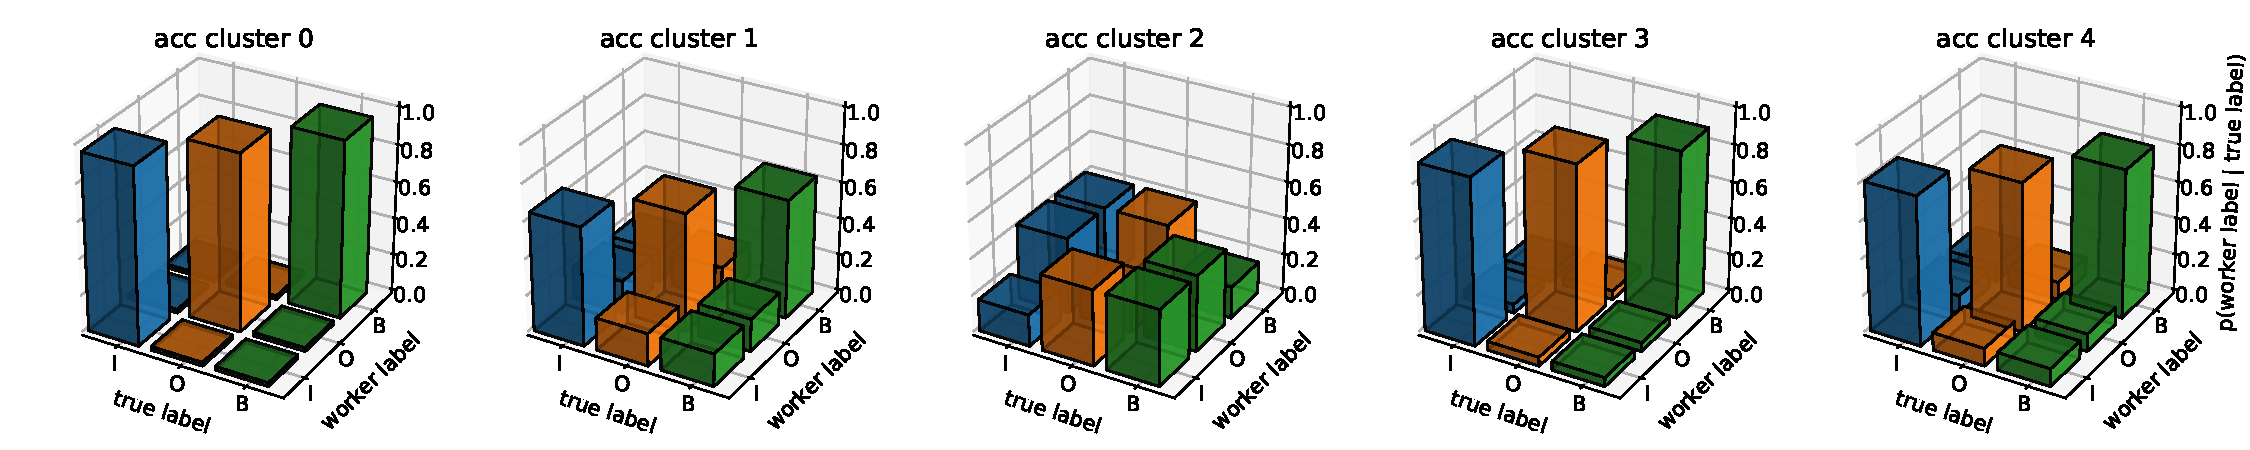
\includegraphics[width=0.9\textwidth, clip=True, trim=0 10 0 27]{figures/worker_models/acc}
% } \\
\subfloat[BSCC-Vec-IF]{
  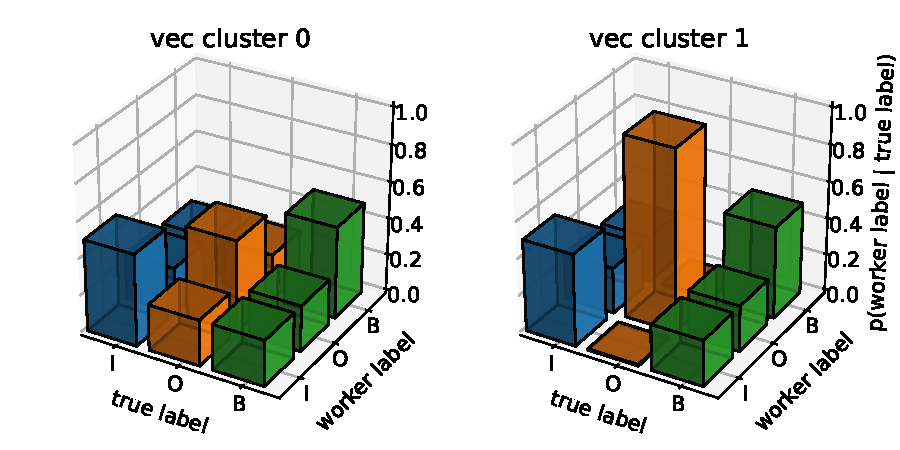
\includegraphics[width=1\textwidth, clip=True, trim=0 10 0 27]{figures/worker_models/vec}
} \\
\subfloat[BSCC-MACE-IF]{
  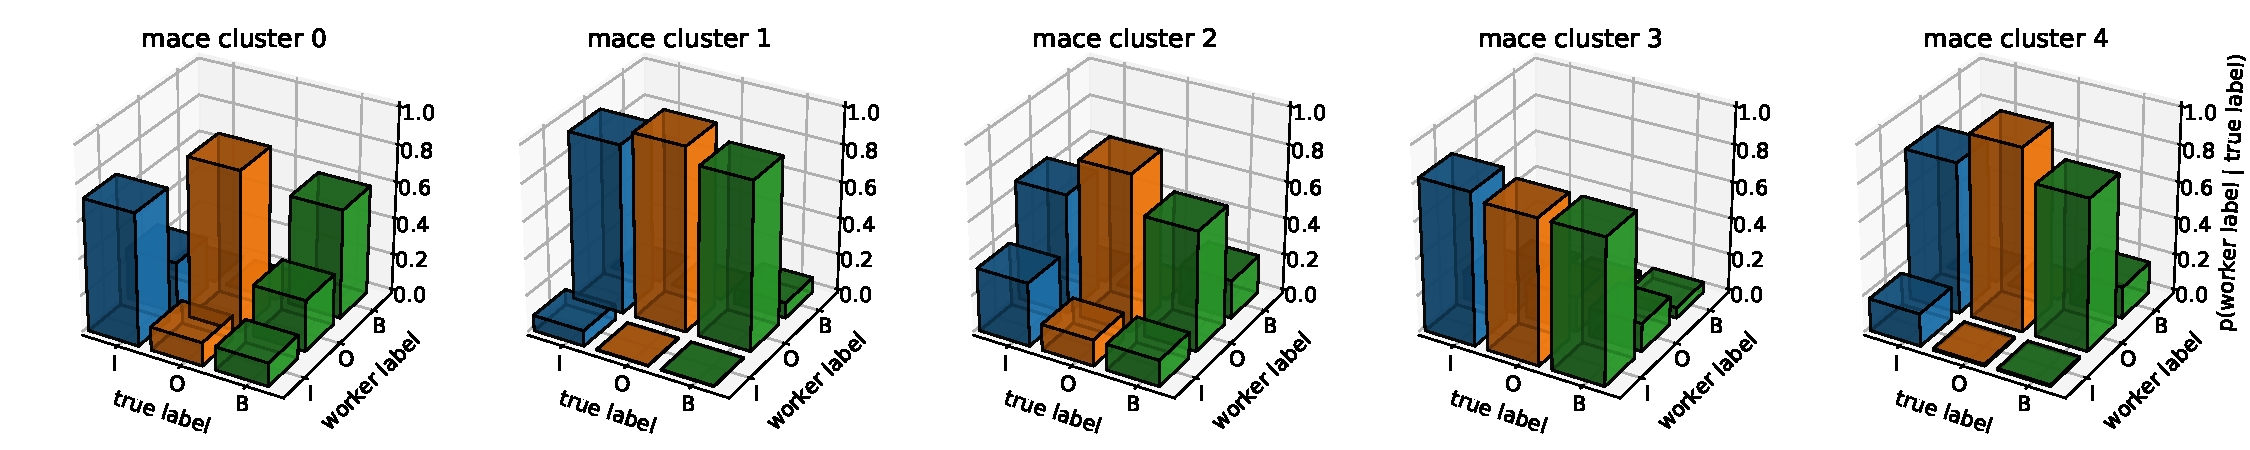
\includegraphics[width=1\textwidth, clip=True, trim=0 10 0 27]{figures/worker_models/mace}
} \\
\subfloat[BSCC-IBCC-IF]{
  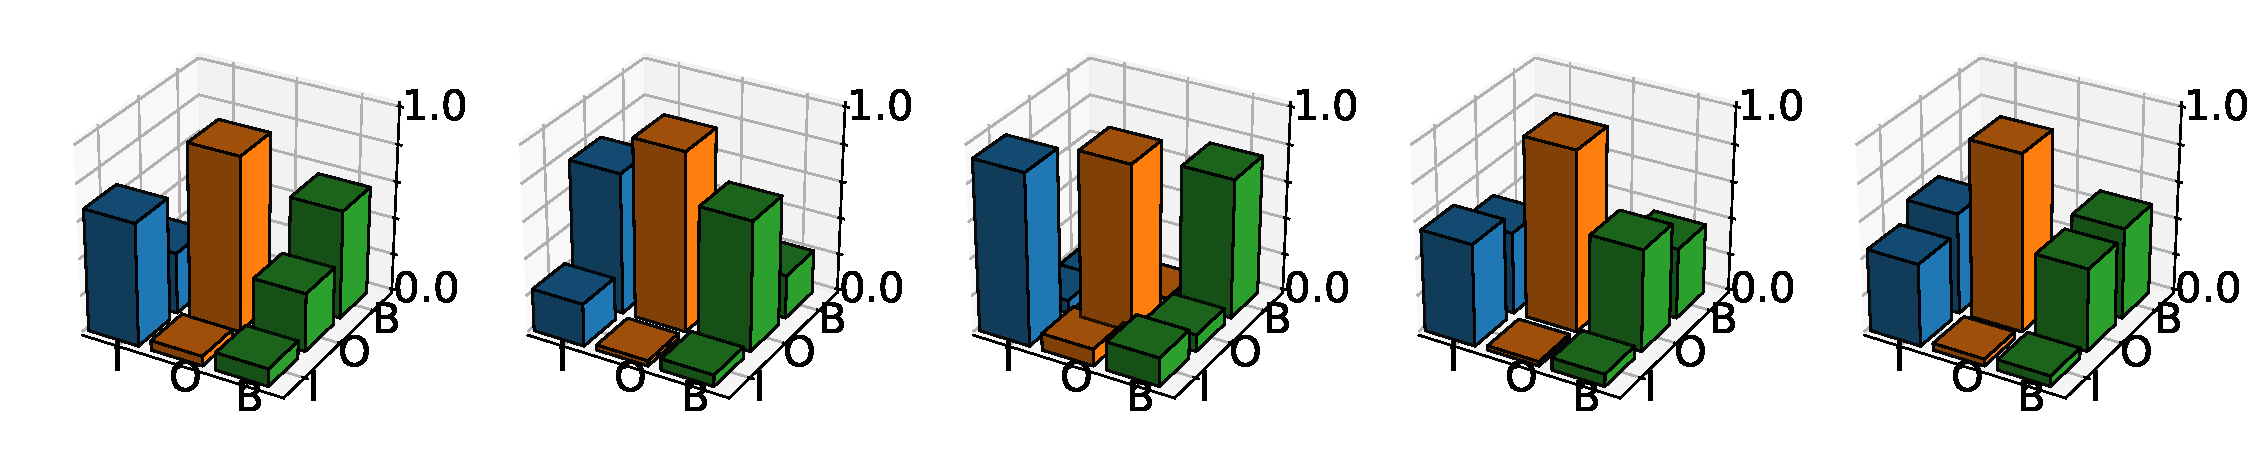
\includegraphics[width=1\textwidth, clip=True, trim=0 10 0 27]{figures/worker_models/ibcc}
} \\
\subfloat[BSCC-seq-IF, previous label = I]{
  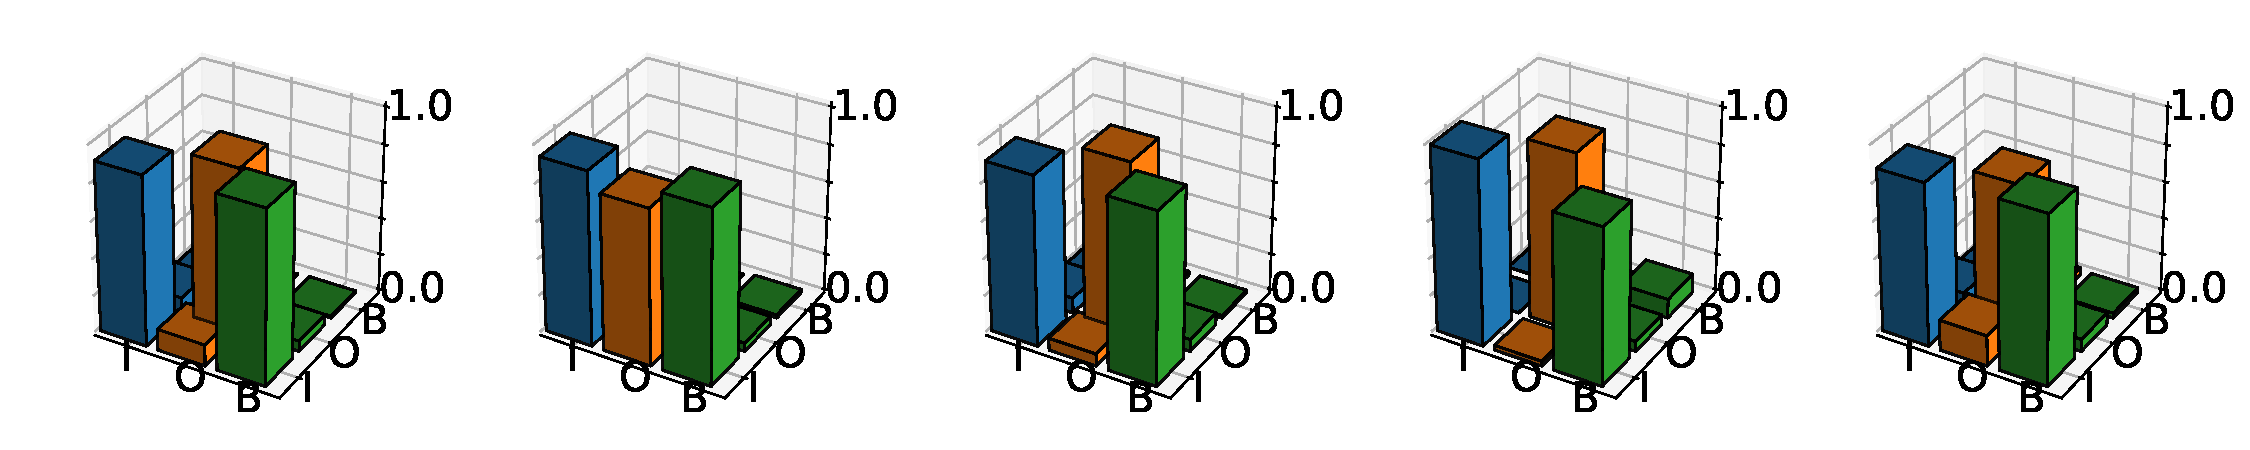
\includegraphics[width=1\textwidth, clip=True, trim=0 10 0 27]{figures/worker_models/seq_prev0}
} \\
\subfloat[BSCC-seq-IF, previous label = O]{
  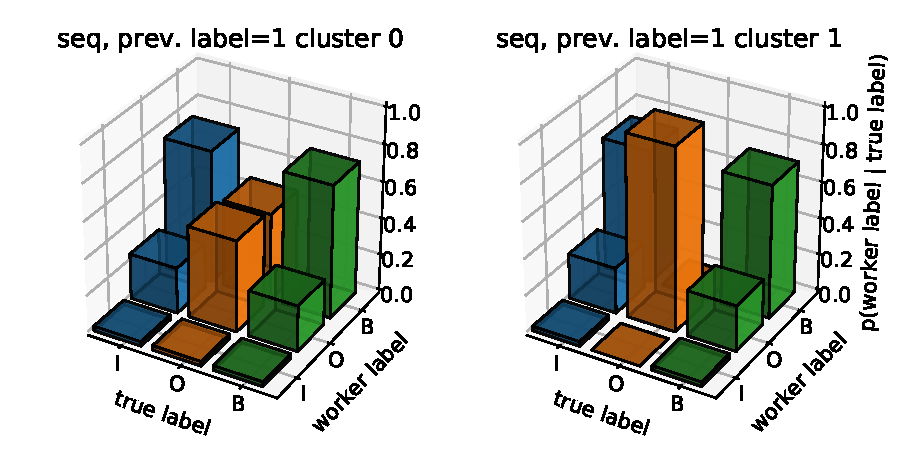
\includegraphics[width=1\textwidth, clip=True, trim=0 10 0 27]{figures/worker_models/seq_prev1}
} \\
\subfloat[BSCC-seq-IF, previous label = B]{
  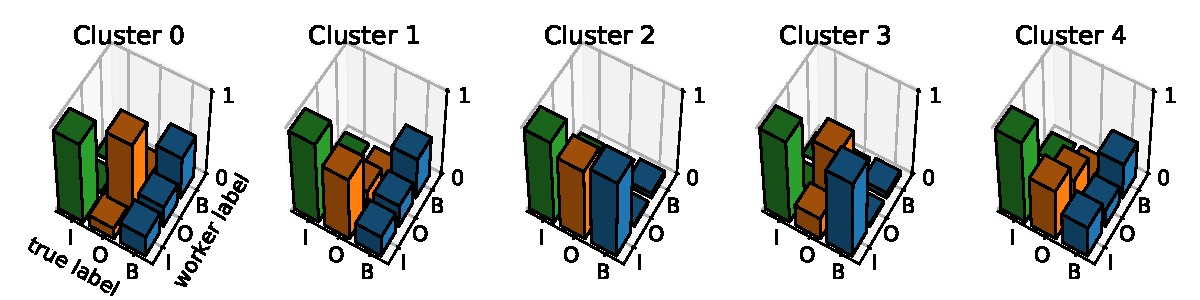
\includegraphics[width=1\textwidth, clip=True, trim=0 10 0 27]{figures/worker_models/seq_prev2}
} \\
\caption{Confusion matrix representations from each BSCC-***-IF variant trained on the PICO datasets 
showing the different representations of workers. 
% Show how worker representation benefits from richer model: e.g. show differences between rows in IBCC compared to acc.
% Represent all types as IBCC-confusion matrix plots. seq will need more >= 3 plots! We can focus on PICO data to make it easier to view,
% or combiner NER classes into BIO. 
% If each row corresponds to one model, we have 7 rows (2 extra for seq). 
% Each row can then show either a selection of 5 workers, or we can cluster into 5 groups.
}
\label{fig:conf_mat_clusters}

\end{figure*}

\begin{figure}
\centering
\subfloat[prev. = I]{
  \includegraphics[width=.31\columnwidth, clip=True, trim=20 47 10 25]{figures/worker_models/seq+LSTM_prev0}
}
\subfloat[prev. = O]{
  \includegraphics[width=.31\columnwidth, clip=True, trim=20 47 10 25]{figures/worker_models/seq+LSTM_prev1}
}
\subfloat[prev. = B]{
  \includegraphics[width=.31\columnwidth, clip=True, trim=20 47 10 25]{figures/worker_models/seq+LSTM_prev2}
}
\caption{PICO dataset: confusion matrices inferred by BSC-Seq-IF+LSTM for the integrated LSTM. }
\label{fig:conf_mat_lstm}
\end{figure}

\subsubsection{Examples of Aggregation}

\begin{figure}
\centering
\subfloat[Example 1]{
  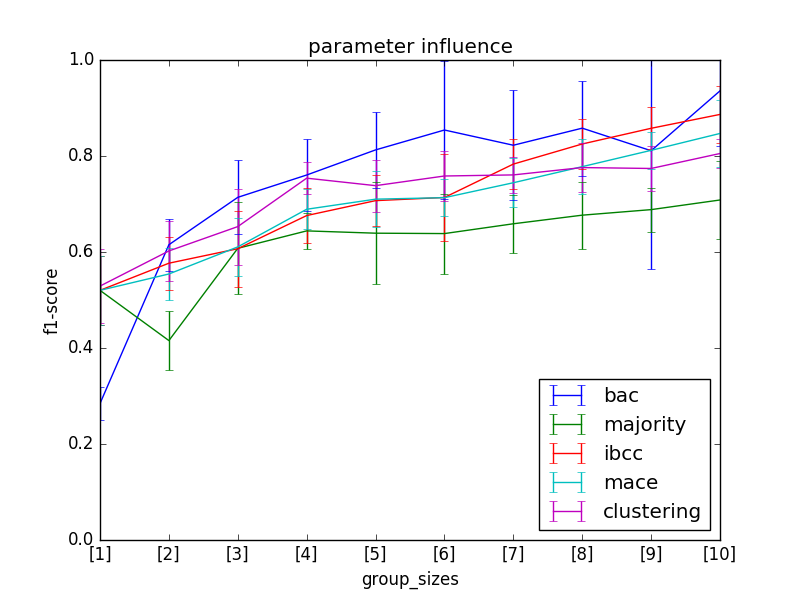
\includegraphics[width=1\columnwidth, clip=True, trim=20 47 10 25]{figures/placeholder}
}\\
\subfloat[Example 2]{
  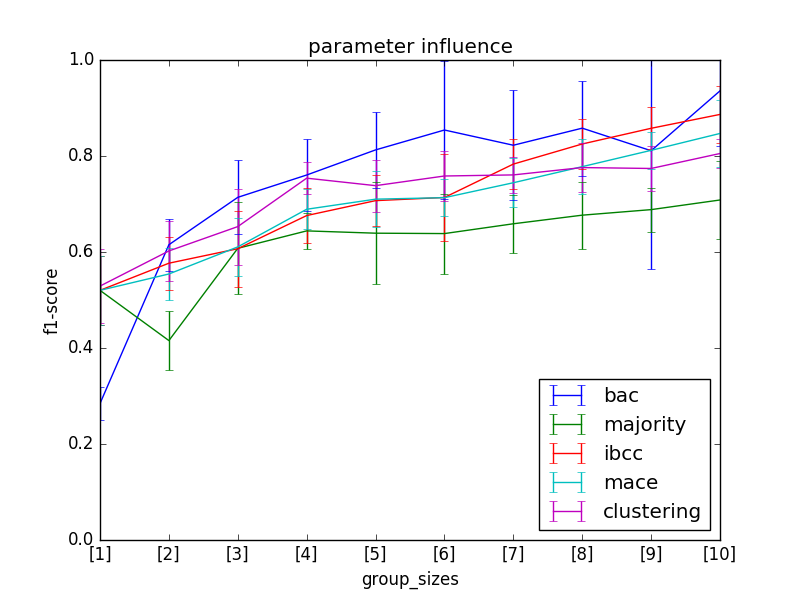
\includegraphics[width=1\columnwidth, clip=True, trim=20 47 10 25]{figures/placeholder}
}\\
\subfloat[Example 3]{
  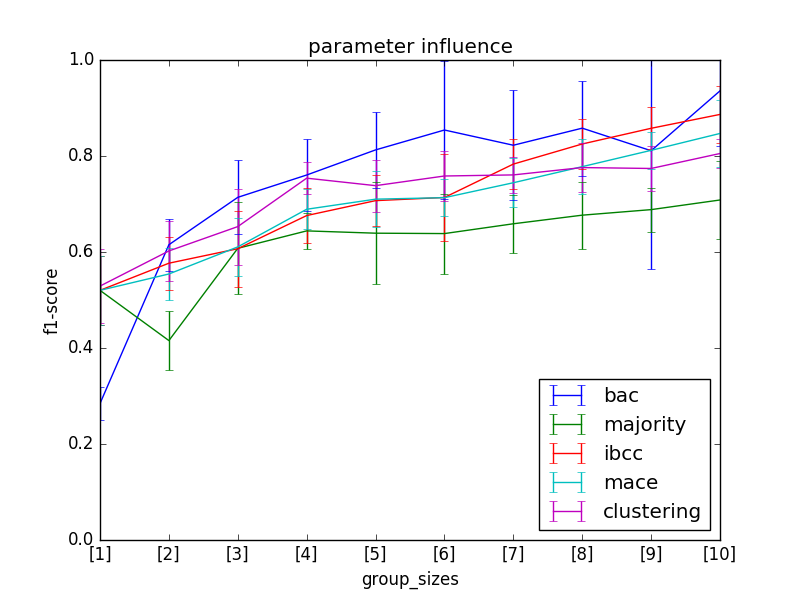
\includegraphics[width=1\columnwidth, clip=True, trim=20 47 10 25]{figures/placeholder}
}
\caption{Examples of different handling of annotator disagreement on PICO. 
Lines above the text show the crowd's annotations. Lines below show the aggregated annotations from MV, IBCC, HMM-Crowd and BSCC-seq-IF.
The sequential methods are able to resolve some issues, 
while non-sequential methods can lead to invalid annotations. }
\label{fig:disagreements}
\end{figure}

\subsection{Prediction using an LSTM Trained by the Crowd}\label{sec:task2}

In this task, we use the aggregation methods to train an LSTM sequence tagger \cite{lample2016}
to show whether integrating the LSTM with the aggregation method improves performance.
For the NER dataset, we train the aggregation methods on the $415$ crowd-labelled documents, as before,
then use the outputs to train the LSTM. We then evaluate the LSTM on the validation and test sets
in the original CoNLL dataset.
With the PICO dataset, we run the aggregators on the $3,649$ documents without gold labels, 
use the outputs to train the LSTM, then evaluate the LSTM on the validation and test splits from the gold-labelled data.


% \begin{table*}
% % \small
% \begin{tabularx}{\textwidth}{| l | Y | Y | Y | Y | Y | Y | Y |}
% \hline
% NER & \multicolumn{3}{|l|}{Span-level metrics}                     & \multicolumn{4}{|l|}{Token-level metrics} \\ \hline 
% & Prec. & Recall & F1 & F1 & AUC & CEE & $N_{inval}$  \\ \hline 
% %HMM-Crowd-then-LSTM & 76.19 & 66.24 & 70.87 &\\ % original results from Nguyen 2017
% %HMM-Crowd-then-LSTM & 72.75 & 68.26 & 70.43 & 35.73 & .8752 & 23.45 & 0 & V. close to Nguyen et al.~\shortcite{nguyen2017aggregating}\\ 
% HMM-crowd$\rightarrow$LSTM & 68.8 & \textbf{65.4} & \textbf{67.1} & \textbf{67.5} & .910 & 15.21 & 1 \\ 
% %LSTM & 83.19 & 57.12 & 67.73 \\ 
% %LSTM-Crowd & 82.38 & 62.10 & 70.82 \\ \hline
% %BSC-seq$\rightarrow$LSTM & \textbf{75.0} & \textbf{68.0} & \textbf{71.3} & \textbf{70.2} & .909 & 13.35 & 0 \\ % this was achieved before the priors were 'fixed' so that the disallowed count from banned transition from restricted_type1 -> restricted_type2 was transferred to unrestricted_type2 instead of restricted_type1. However, the method without LSTM improved...
% BSC-seq$\rightarrow$LSTM & \textbf{71.5} & 59.3 & 64.9 & 66.7 & .867 & 17.43 & 0 \\  
% %BSC-seq+LSTM & 71.7 & 62.7 & 66.9 & 65.9 & \textbf{.957} & \textbf{0.542} & 0 \\
% BSC-seq+LSTM & 69.3 & 61.1 & 64.9 & 66.3 & \textbf{.945} & \textbf{0.89} & 0 \\  
% %BCC-seq+LSTM & 39.7 & 14.1 & 20.9 & 31.6 & .924 & 2.14 & 0 \\
% \hline
% \end{tabularx}
% \caption{Prediction performance on NER test dataset with training on crowdsourced labels.}
% \label{tab:prediction_results_ner}
% \end{table*}
%
\begin{table*}
% \small
\begin{tabularx}{\textwidth}{| l | Y | Y | Y | Y | Y | Y | Y |}
\hline
NER & \multicolumn{3}{|l|}{Span-level metrics}                     & \multicolumn{4}{|l|}{Token-level metrics} \\ \hline 
& Prec. & Recall & F1 & F1 & AUC & CEE & $N_{inval}$  \\ \hline 
MV$\rightarrow$LSTMd & 69.4 & 55.1 & 61.5 & 66.0 & .8775 & 19.48 & 0 \\
IBCC$\rightarrow$LSTMd & 77.6 & 55.7 & 64.9 & 64.8 & .8555 & 17.96 & 44 \\
\hline
HMM-crowd$\rightarrow$LSTMp & 77.0 & 58.2 & 66.3 & 70.2 & .9911 & 0.23 & 407 \\ 
HMM-crowd$\rightarrow$LSTMd & 78.7 & 59.0 & 67.5 & 69.4 & .8642 & 15.88 & 0 \\ 
%LSTM & 83.19 & 57.12 & 67.73 \\ 
%LSTM-Crowd & 82.38 & 62.10 & 70.82 \\ \hline
BSC-seq$\rightarrow$LSTMp & 72.9 & 62.4 & 67.2 & 69.3 & .9908 & 0.22 & 0 \\  
BSC-seq$\rightarrow$LSTMd & 74.3 & 62.8 & 68.1 & 69.7 & .8868 & 15.65 & 0 \\  
BSC-seq+LSTMp & 74.4 & 60.3 & 66.6 & 68.2 & .9782 & 0.33 & 0 \\  
BSC-seq+LSTMd & 73.4 & 62.0 & 67.3 & 67.6 & .9589 & 0.48 & 0 \\
\hline
gold$\rightarrow$LSTMp & 74.0 & 75.1 & 74.5 & 76.0 & .9945 & 0.19 & 105 \\
gold$\rightarrow$LSTMd & 76.4 & 77.0 & 76.7 & 77.3 & .9563 & 11.10 & 3 \\
\hline
\end{tabularx}
\caption{Prediction performance on NER test dataset with training on crowdsourced labels.}
\label{tab:prediction_results_ner}
\end{table*}
%
\begin{table*}
% \small
\begin{tabularx}{\textwidth}{| l | Y | Y | Y | Y | Y | Y | Y |}
\hline
PICO & \multicolumn{3}{|l|}{Span-level metrics (std.)}                          & \multicolumn{4}{|l|}{Token-level metrics (std.)} \\ \hline 
& Prec. & Recall & F1 & F1 & AUC & CEE & $N_{inval}$ \\ \hline
HMM-Crowd$\rightarrow$LSTMd & \textbf{75.6} & 61.6 & 67.9 & \textbf{76.4} & .8380 & 13.46 & 0\\ \hline
BSC-seq$\rightarrow$LSTMd & 74.0 & \textbf{66.1} & \textbf{69.8} & 58.2 & .8349 & 19.62 & 0 \\
BSC-seq+LSTM & 60.7 & 52.8 & 56.4 & 54.0 & \textbf{.899} & \textbf{0.48} & 0\\
%BCC-seq+LSTM &\\
\hline
\end{tabularx}
\caption{Prediction performance on PICO test dataset with training on crowdsourced labels.}
\label{tab:prediction_results_pico}
\end{table*}


\section{Active Document Selection}

We run an active learning simulation to evaluate whether the proposed Bayesian approach and integrated LSTM
can improve the efficiency of the crowdsourcing process. 
The simulation is run separately for each method tested, and begins with the same initial set of randomly-chosen
documents taken from the same crowd-labelled sets used in Section \ref{sec:task2}.
We retrieve the crowdsourced labels for the selected documents, run the aggregation method,
then use its posterior probabilities to select a new batch of the $N_{batchsize}$ most uncertain documents that have not yet been labelled. 
We retrieve the annotations for the selected batch of documents, then repeat the process until
all of the availble crowd labels have been used.
We set $N_{batchsize}$ to one tenth of the crowd-labelled dataset size for each of the datasets. At each iteration,
we monitor progress by training an LSTM on the current output of the aggregation method, 
and testing its performance as in Section \ref{sec:task2}. 
With the NER dataset we also evaluate the output of aggregation method on the test set for the crowd-labelled documents. 
This is not possible with PICO datas because we do not have gold labels for documents labelled by the crowd.

The active learning process tested here employs \emph{uncertainty sampling}, which is a well-established heuristic \cite{active learning paper -- see tacl paper?}. The selection method and batch size could be fine-tuned for future applications -- the goal of our experiment in this paper was to test the benefits of the proposed aggregation methods,
rather than to establish a robust active learning approach.
 
\begin{figure}
\centering
% \subfloat[NER dataset]{
  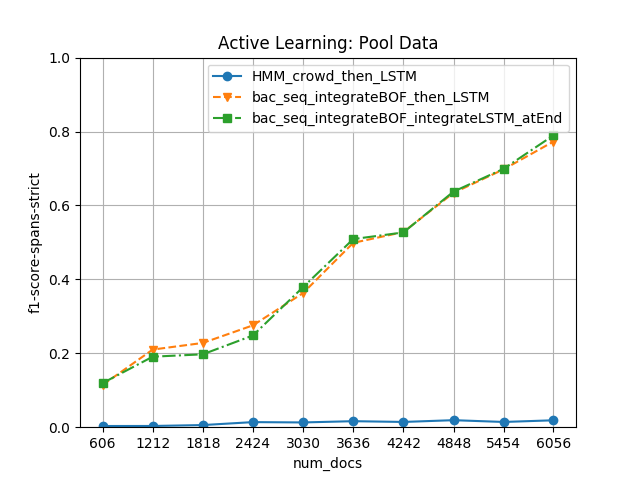
\includegraphics[width=1\columnwidth, clip=True, trim=35 0 40 40]{figures/NER_AL/pool/plot_f1-score-spans-strict.png}
% }
% \subfloat[PICO dataset]{
%   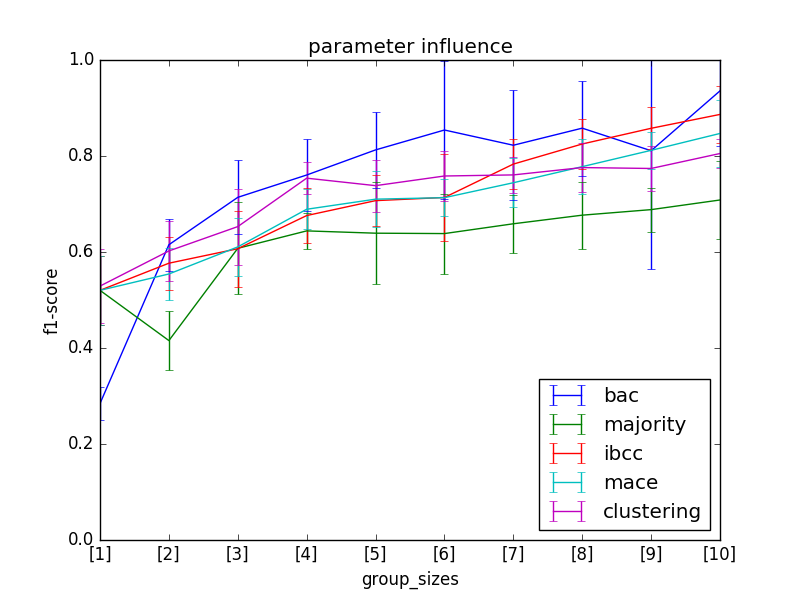
\includegraphics[width=.7\columnwidth, clip=True, trim=20 47 10 25]{figures/placeholder}
% }
\caption{Active learning simulation with NER dataset: increasing span-level F1-score.
%: prediction performance after each labelled batch is received. Mean scores over 10 repeats.
}
\label{fig:al}
\end{figure}

\section{Discussion}

The benefits of sequential models are more evident on the PICO dataset than on NER, which may be due to the longer sequences or the smaller number of labels, since PICO target classes are only B, I, or O, whereas the B and I tags for NER 
are compounded with PER, LOC, ORG or MISC tags. <show an example from each dataset, with our predictions from HMM, BAC...>
